
\documentclass{beamer}

\mode<presentation> {

% The Beamer class comes with a number of default slide themes
% which change the colors and layouts of slides. Below this is a list
% of all the themes, uncomment each in turn to see what they look like.

%\usetheme{default}
%\usetheme{AnnArbor}
%\usetheme{Antibes}
%\usetheme{Bergen}
%\usetheme{Berkeley}
%\usetheme{Berlin}
%\usetheme{Boadilla}
%\usetheme{CambridgeUS}
%\usetheme{Copenhagen}
%\usetheme{Darmstadt}
%\usetheme{Dresden}
%\usetheme{Frankfurt}
%\usetheme{Goettingen}
%\usetheme{Hannover}
%\usetheme{Ilmenau}
%\usetheme{JuanLesPins}
%\usetheme{Luebeck}
\usetheme{Madrid}
%\usetheme{Malmoe}
%\usetheme{Marburg}
%\usetheme{Montpellier}
%\usetheme{PaloAlto}
%\usetheme{Pittsburgh}
%\usetheme{Rochester}
%\usetheme{Singapore}
%\usetheme{Szeged}
%\usetheme{Warsaw}

% As well as themes, the Beamer class has a number of color themes
% for any slide theme. Uncomment each of these in turn to see how it
% changes the colors of your current slide theme.

%\usecolortheme{albatross}
%\usecolortheme{beaver}
%\usecolortheme{beetle}
%\usecolortheme{crane}
%\usecolortheme{dolphin}
%\usecolortheme{dove}
%\usecolortheme{fly}
%\usecolortheme{lily}
%\usecolortheme{orchid}
%\usecolortheme{rose}
%\usecolortheme{seagull}
%\usecolortheme{seahorse}
%\usecolortheme{whale}
%\usecolortheme{wolverine}

%\setbeamertemplate{footline} % To remove the footer line in all slides uncomment this line
%\setbeamertemplate{footline}[page number] % To replace the footer line in all slides with a simple slide count uncomment this line

%\setbeamertemplate{navigation symbols}{} % To remove the navigation symbols from the bottom of all slides uncomment this line
}

\usepackage[utf8]{inputenc}
\usepackage[T1]{fontenc}
\usepackage[english]{babel}
\usepackage{graphicx} % Allows including images
\usepackage{booktabs} % Allows the use of \toprule, \midrule and \bottomrule in tables
\usepackage{listings}
\usepackage{mathtools}

\usepackage{subcaption}
\renewcommand{\familydefault}{\rmdefault}

%----------------------------------------------------------------------------------------
%	TITLE PAGE
%----------------------------------------------------------------------------------------

\title[CPU cache - SRAM]{CPU cache - MOSFET 6T SRAM} % The short title appears at the bottom of every slide, the full title is only on the title page

\author{Marcus Malmquist} % Your name
\institute[Chalmers] % Your institution as it will appear on the bottom of every slide, may be shorthand to save space
{
Chalmers University of Technology \\ % Your institution for the title page
\medskip
\textit{marmalm@student.chalmers.se} % Your email address
}
\date{\today} % Date, can be changed to a custom date

\begin{document}

\begin{frame}
\titlepage % Print the title page as the first slide
\end{frame}

%----------------------------------------------------------------------------------------
%	PRESENTATION SLIDES
%----------------------------------------------------------------------------------------

\begin{frame}
  \frametitle{What is CPU cache?}
  \begin{itemize}
  \item Dedicated CPU memory.
  \item Resides on the CPU.
  \item Fast (same clock rate as CPU).
  \item Volatile (data is lost when power is cut).
  \item Static RAM technology (not to be confused with Synchronous RAM used as the main memory).
  \item Very expensive.
  \item Very small compared to main memory (kilobytes for L1 cache and megabytes for L2 cache).
  \end{itemize}
\end{frame}

\begin{frame}
  \frametitle{Why is it fast?}
  \begin{itemize}
  \item Being physically located on the CPU means short access times (the CPU does not need to access it through the chipset).
  \item Small in physical size and storage capacity means short access time for each cell.
  \item Static RAM (used in cache) uses flip-flop (two steady states) which is faster is faster than Dynamic RAM (used as main memory) which uses capacitors to store bits.
  \end{itemize}
\end{frame}

\begin{frame}
  \frametitle{How does it work?}
  \begin{itemize}
  \item Typically made up of SRAM cells of six MOSFETs.
  \item Each bit is stored using four transistors while the other two are used for read/write access.
  \item \textbf{Acces} a cell by turning on the word line.
  \item \textbf{Write} by sending the bit down the bit line and the inverse bit down the inverse bit line (\#).
  \item \textbf{Read} by observing what comes out from the bit lines.
  \end{itemize}
  \begin{figure}
    \noindent\makebox[\textwidth]{\scalebox{0.7}{\input{figures/sdram_t.pdf_t}}}
  \end{figure}
\end{frame}

\begin{frame}
  \frametitle{How does it work?}
  \begin{itemize}
  \item Sample implementation from -98 by Fujitsu Ltd.
  \end{itemize}
  \begin{figure}
    \begin{subfigure}{0.49\textwidth}
      \centering
      \noindent\makebox[\textwidth]{\scalebox{1}{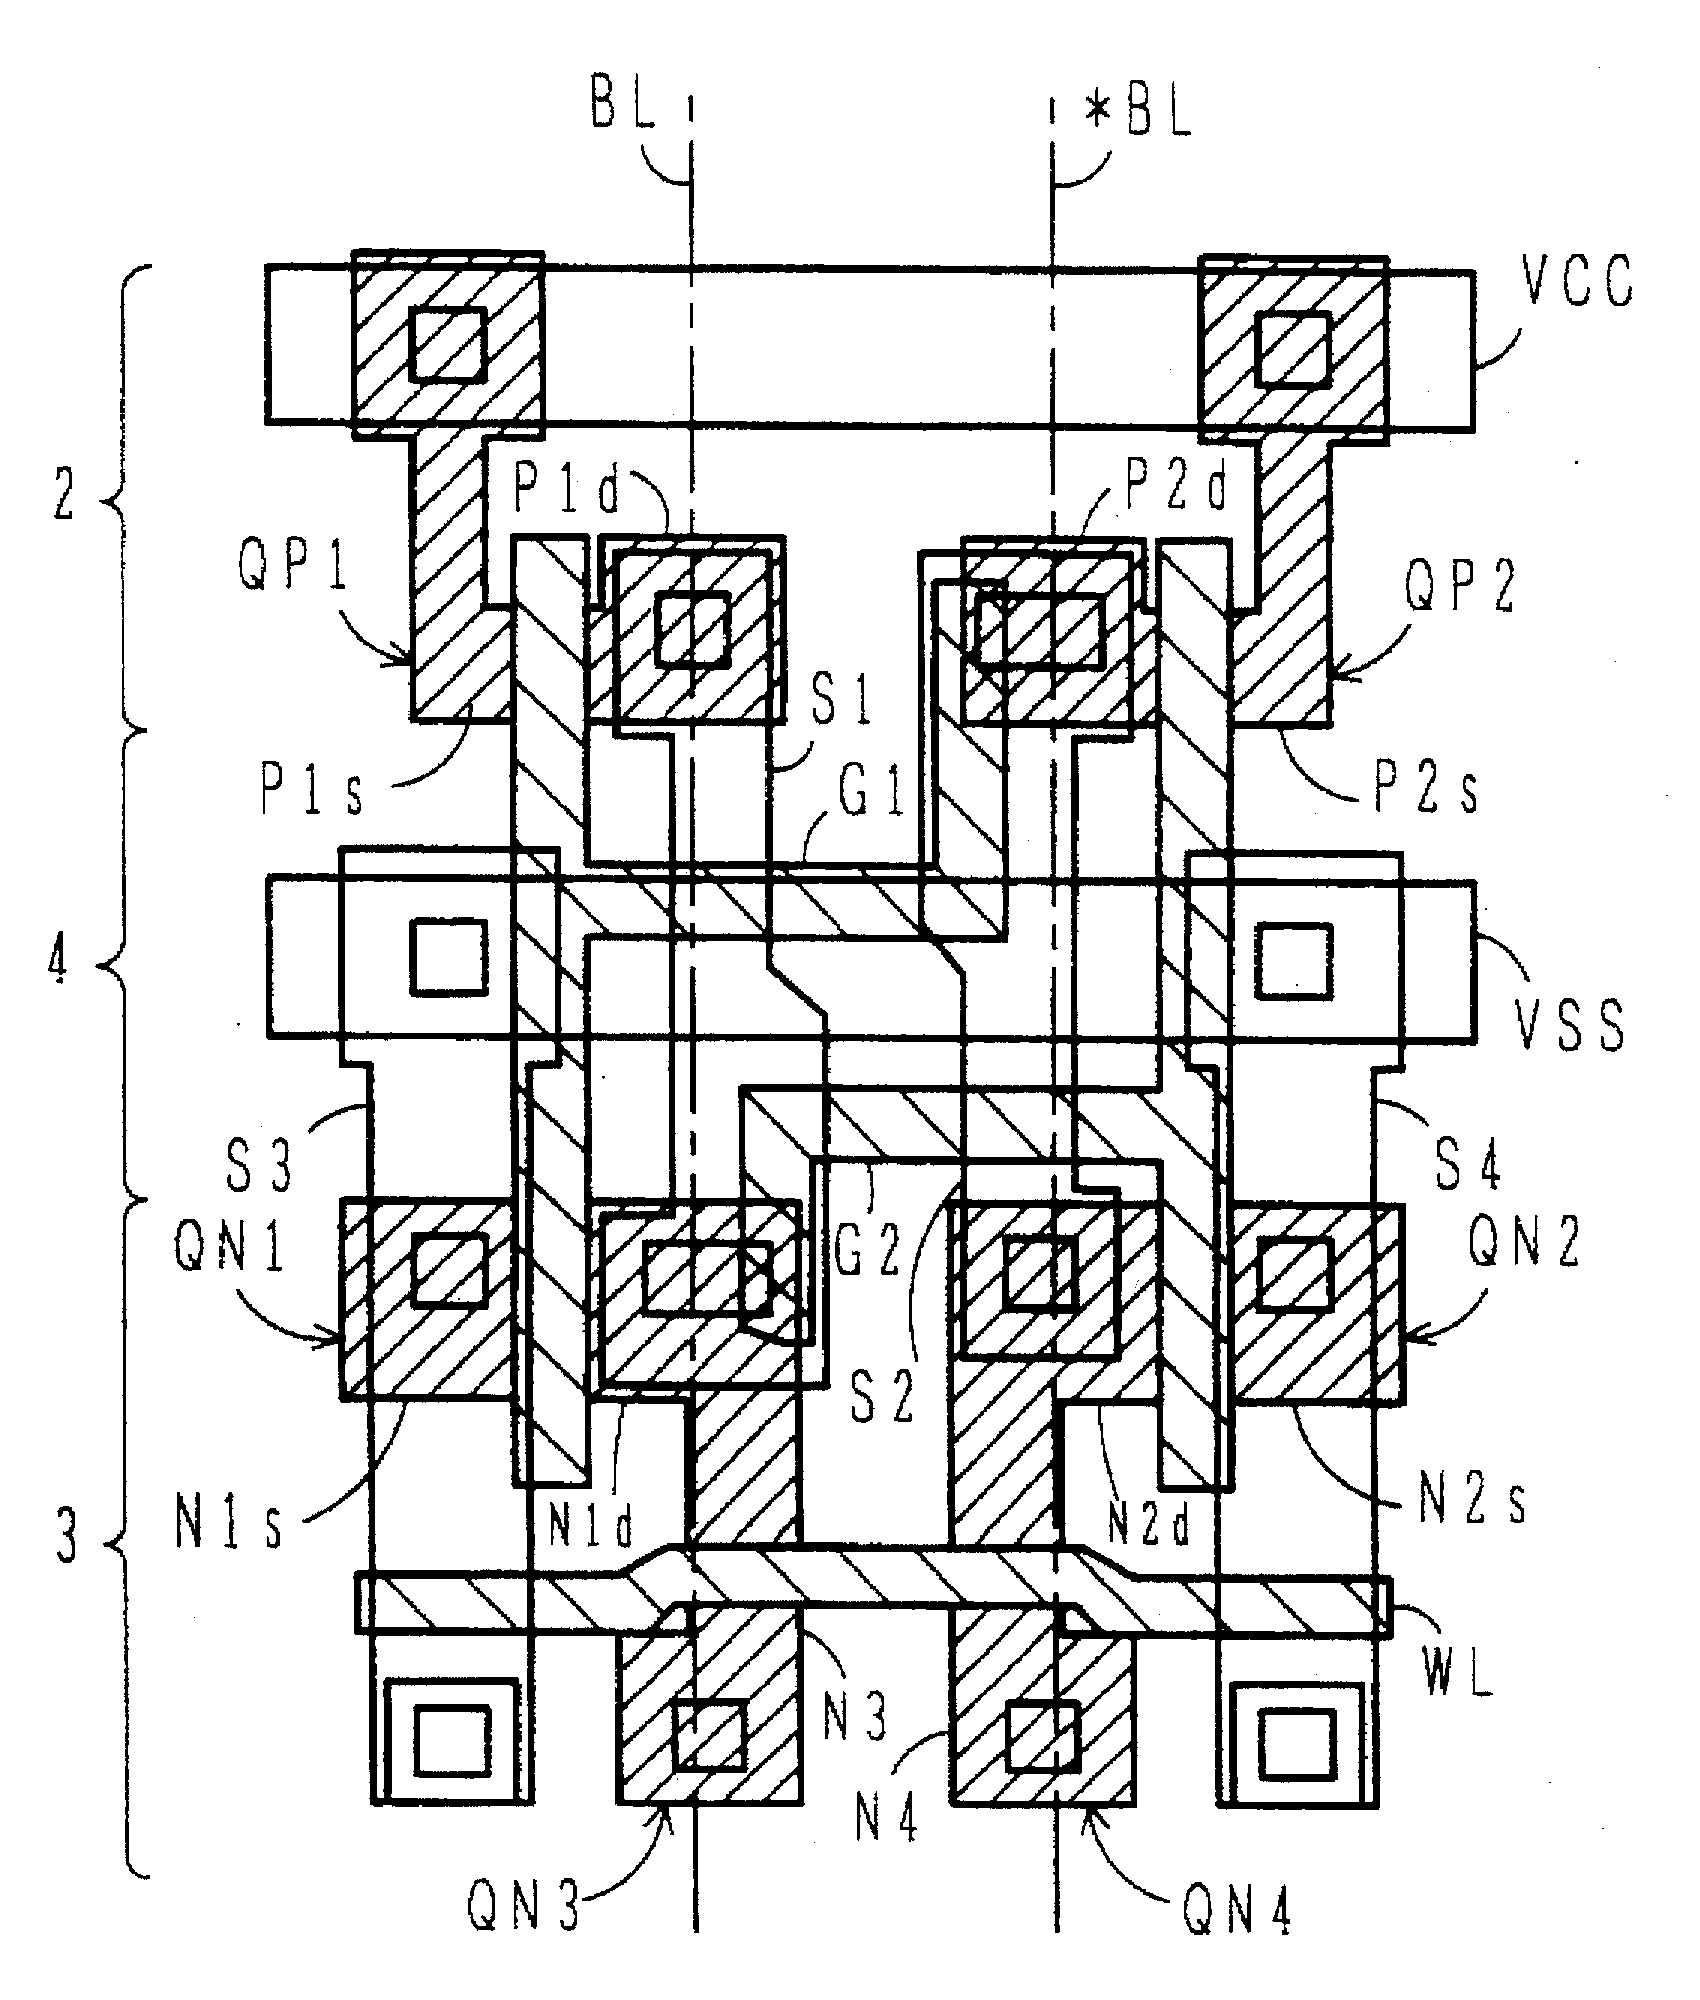
\includegraphics[width=\textwidth]{figures/10.png}}}
    \end{subfigure}
    \begin{subfigure}{0.49\textwidth}
      \centering
      \noindent\makebox[\textwidth]{\scalebox{1}{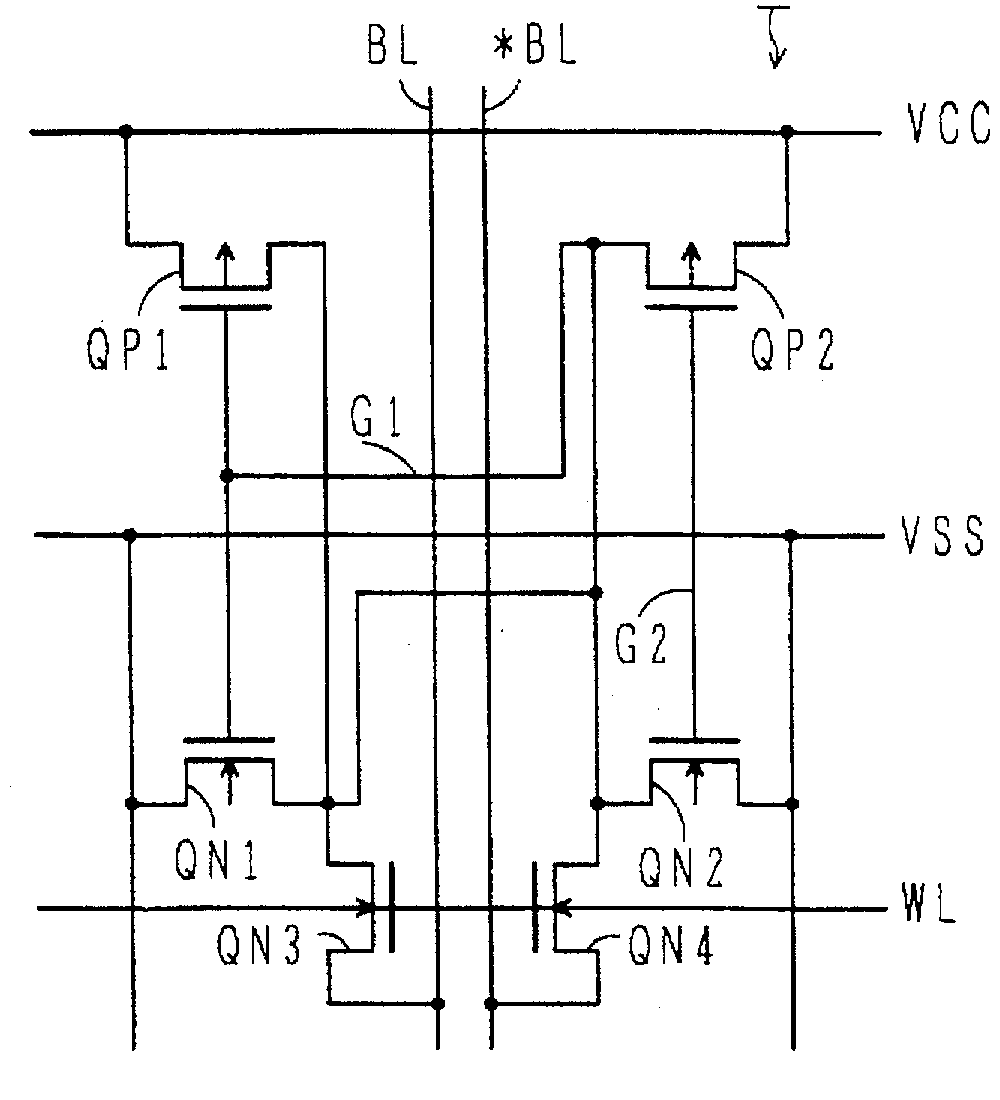
\includegraphics[width=\textwidth]{figures/11a.png}}}
    \end{subfigure}
  \end{figure}
\end{frame}

\begin{frame}
  \frametitle{How does it work}
  \begin{itemize}
  \item Same basic 6T MOSFET flip-flop is used.
  \item Figure shows a 6T SRAM Cell in Intel CORE i5-3550 (2012).
  \item Features tri-gate transistors (the vertical metal gates are not shown in the figure).
  \end{itemize}
  \begin{columns}[c]
    \column{.5\textwidth} % Right column and width
    \begin{itemize}
    \item N1 and N2 are Pull-down NMOS (equivalent of QN1 and QN2 from previous slide).
    \item P1 and P2 are Pull-up PMOS (equivalent of QP1 and QP2 from previous slide).
    \item N3 and N4 are Access-control NMOS (equivalent of QN3 and QN4 from previous slide).
    \end{itemize}
    
    \column{.45\textwidth} % Left column and width
    \begin{figure}
      \noindent\makebox[\textwidth]{\scalebox{1}{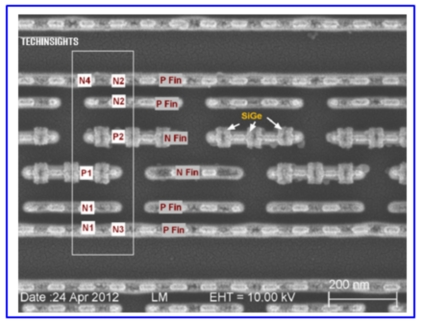
\includegraphics[width=\textwidth]{figures/120906_intel_22_2.png}}}
    \end{figure}
  \end{columns}
\end{frame}

%------------------------------------------------

\begin{frame}
  \frametitle{Example 1}
  \begin{itemize}
  \item Explain how the order of the loops impact execution time for the two methods. \texttt{arr} is a block of contiguous memory with \texttt{rows} x \texttt{cols} elements.
  \end{itemize}
  \begin{block}{10 ms for a 1000x1000 matrix, 2700 ms for a 20000x20000 matrix}
    \tiny\texttt{\lstinputlisting[language=C]{fast.c}}
  \end{block}
  \begin{block}{10 ms for a 1000x1000 matrix, 15400 ms for a 20000x20000 matrix}
    \tiny\texttt{\lstinputlisting[language=C]{slow.c}}
  \end{block}
\end{frame}

\begin{frame}
  \frametitle{Solution 1}
  
  \begin{columns}[c]
    \column{.45\textwidth} % Right column and width
    \begin{itemize}
    \item Each row is a contiguous block of memory.
    \item The element after $(k,n)$ in memory is $(k+1,1)$.
    \end{itemize}
    \column{.5\textwidth} % Left column and width
    \begin{figure}
      \noindent\makebox[\textwidth]{\scalebox{0.7}{\input{figures/example1.pdf_t}}}
    \end{figure}
  \end{columns}
  \begin{itemize}
  \item A 1000x1000 matrix of type double uses 7.6 MB of memory.
    \begin{itemize}
    \item Copying contiguous memory to cache is possible for both methods.
    \item Few cache misses for both methods.
    \end{itemize}
  \item A 20000x20000 matrix of type double uses 3.0 GB of memory.
    \begin{itemize}
    \item Copying contiguous memory to cache is possible for the fast method.
    \item Few cache misses for the fast method.
    \item Copying contiguous memory to cache not possible for the slow method.
    \item Many cache misses for the slow method.
    \end{itemize}
  \end{itemize}
\end{frame}

\begin{frame}
  \frametitle{References}
  \footnotesize{
    \begin{thebibliography}{99} % Beamer does not support BibTeX so references must be inserted manually as below
    \bibitem[higuchi]{p1} Tsuyoshi Higuchi, Fujitsu Limited (1998)
      \newblock CMOS SRAM cell, US 5744844 A
      \newblock \url{https://docs.google.com/viewer?url=patentimages.storage.googleapis.com/pdfs/US5744844.pdf}

    \bibitem[wikipedia]{p1} Various, accessed 2017-10-03
      \newblock Static random-access memory
      \newblock \url{https://en.wikipedia.org/wiki/Static_random-access_memory}

    \bibitem[embedded]{p1} Arabinda Das and Alexandre Dorofeev, Senior Technology Analysts, UBM TechInsights
      \newblock Intel's 22-nm process gives MOSFET switch a facelift
      \newblock \url{https://www.embedded.com/print/4395587}
    \end{thebibliography}
  }
\end{frame}
\begin{frame}
  \Huge{\centerline{The End}}
\end{frame}

\end{document} 